\section{Appendix}

\begin{figure*}[!htb]
	\centering
	% \hspace*{-5mm}
	\subfloat[]{
		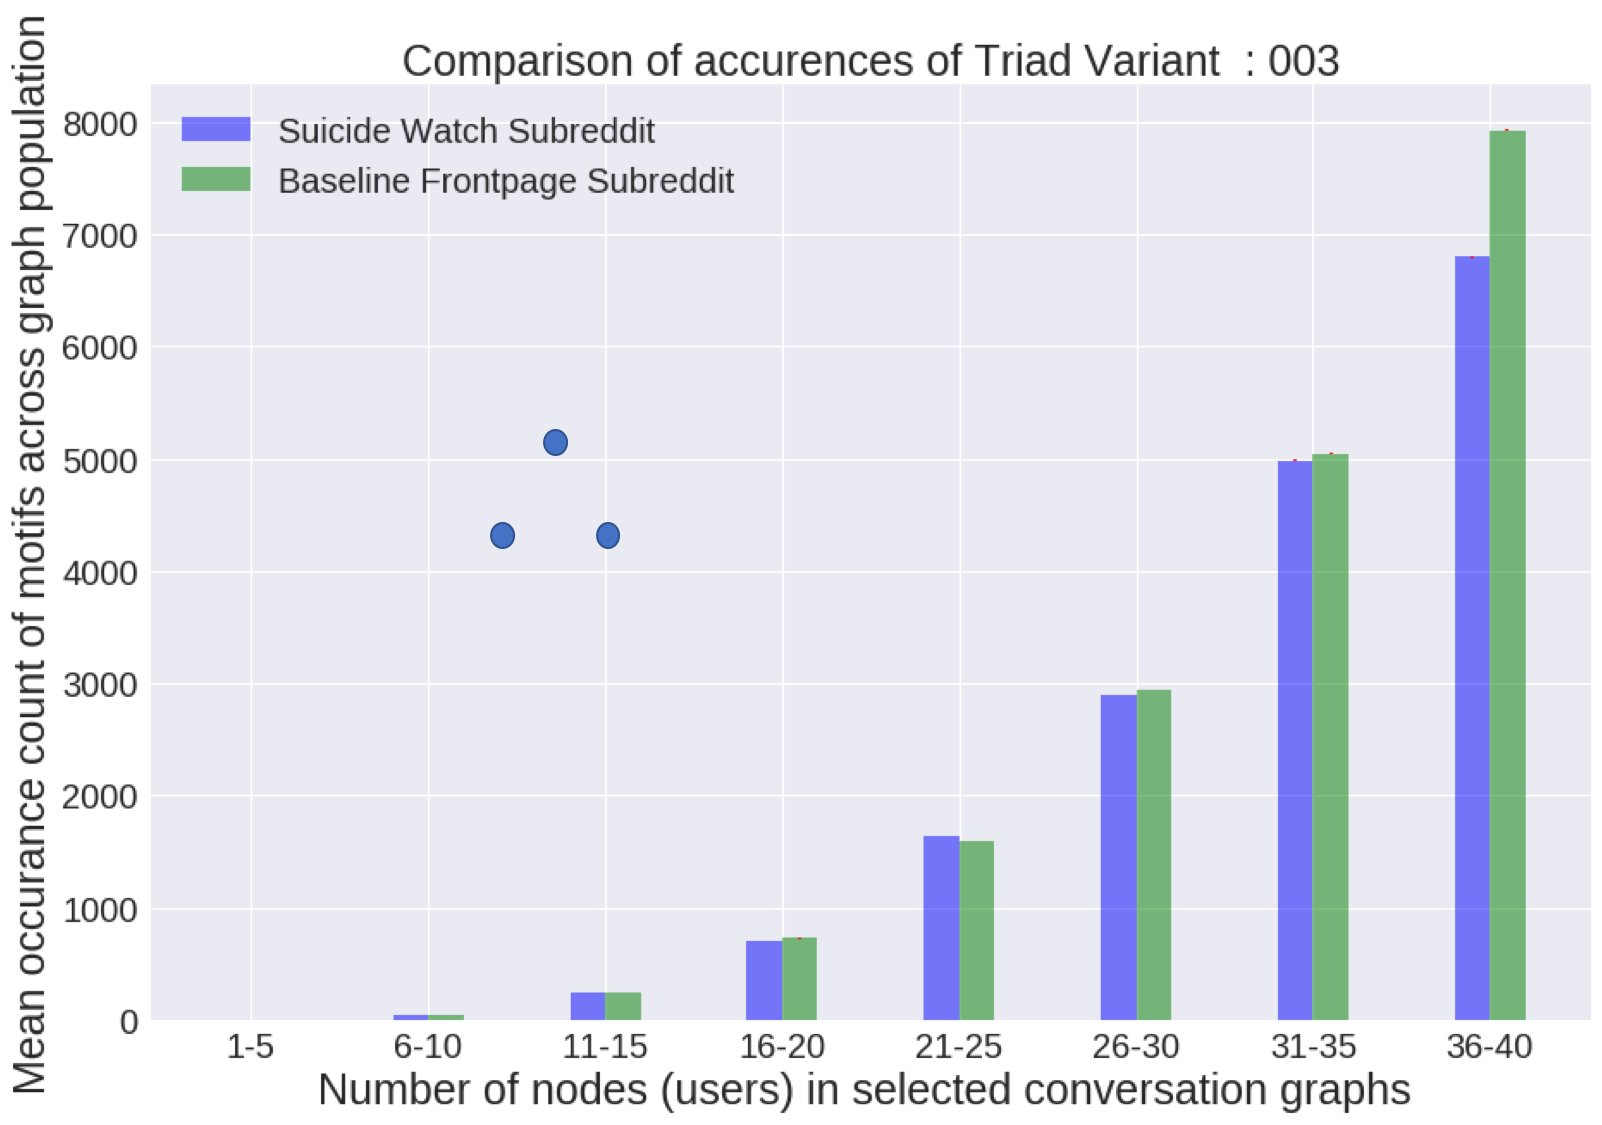
\includegraphics[width=0.33\textwidth, height = 4.5cm ]{Figures/003}
		\label{fig:003}
	}
	\subfloat[]{
		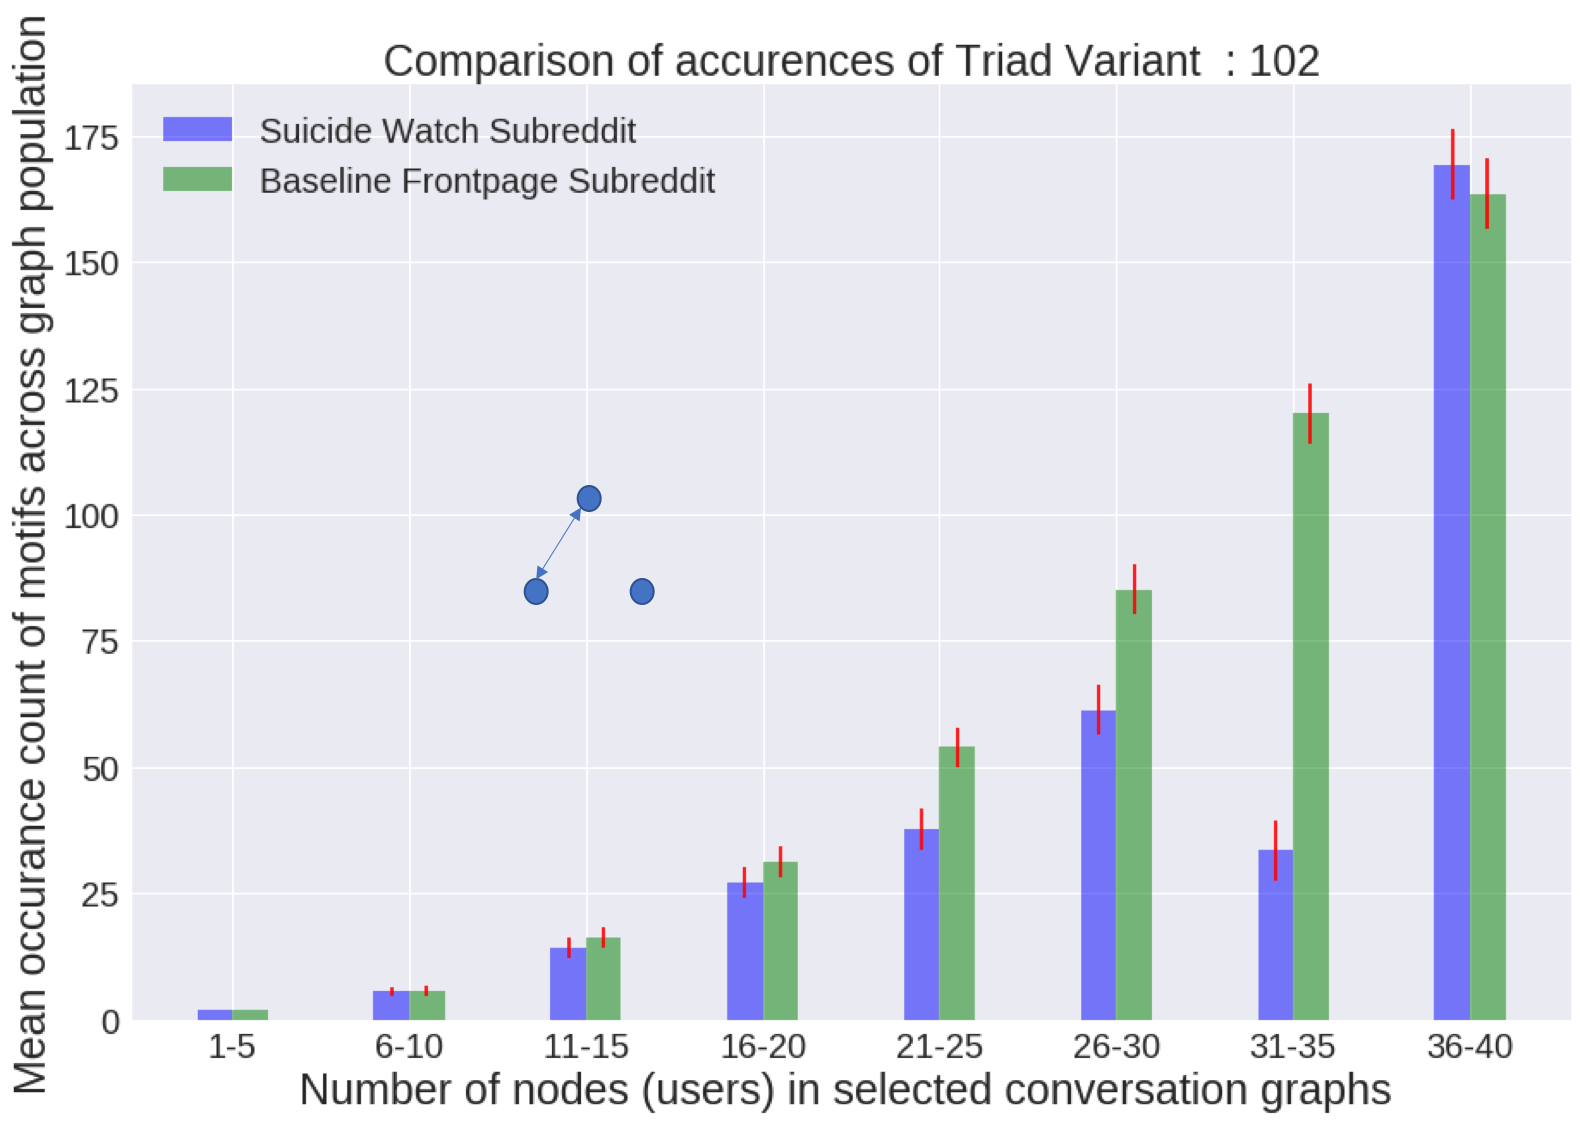
\includegraphics[width=0.33\textwidth, height = 4.5cm ]{Figures/102}
		\label{fig:102}
	}
	\subfloat[]{
		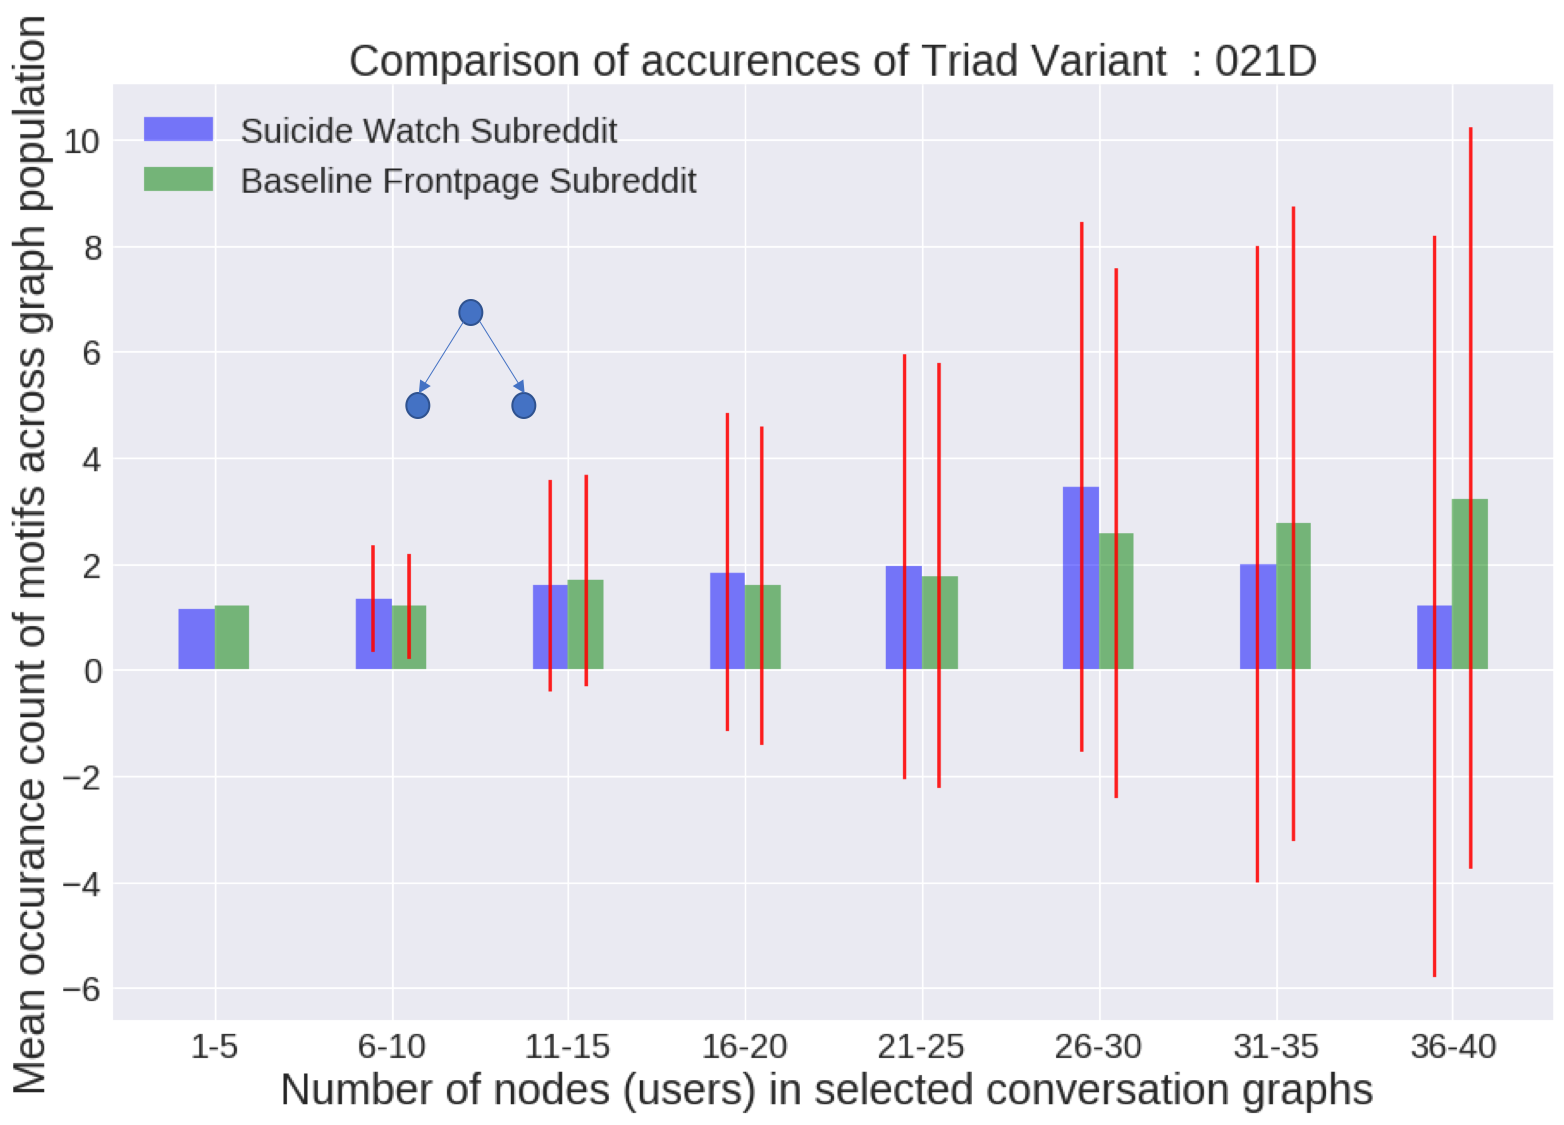
\includegraphics[width=0.33\textwidth, height = 4.5cm ]{Figures/021D}
		\label{fig:021D}
	}


	\subfloat[]{
	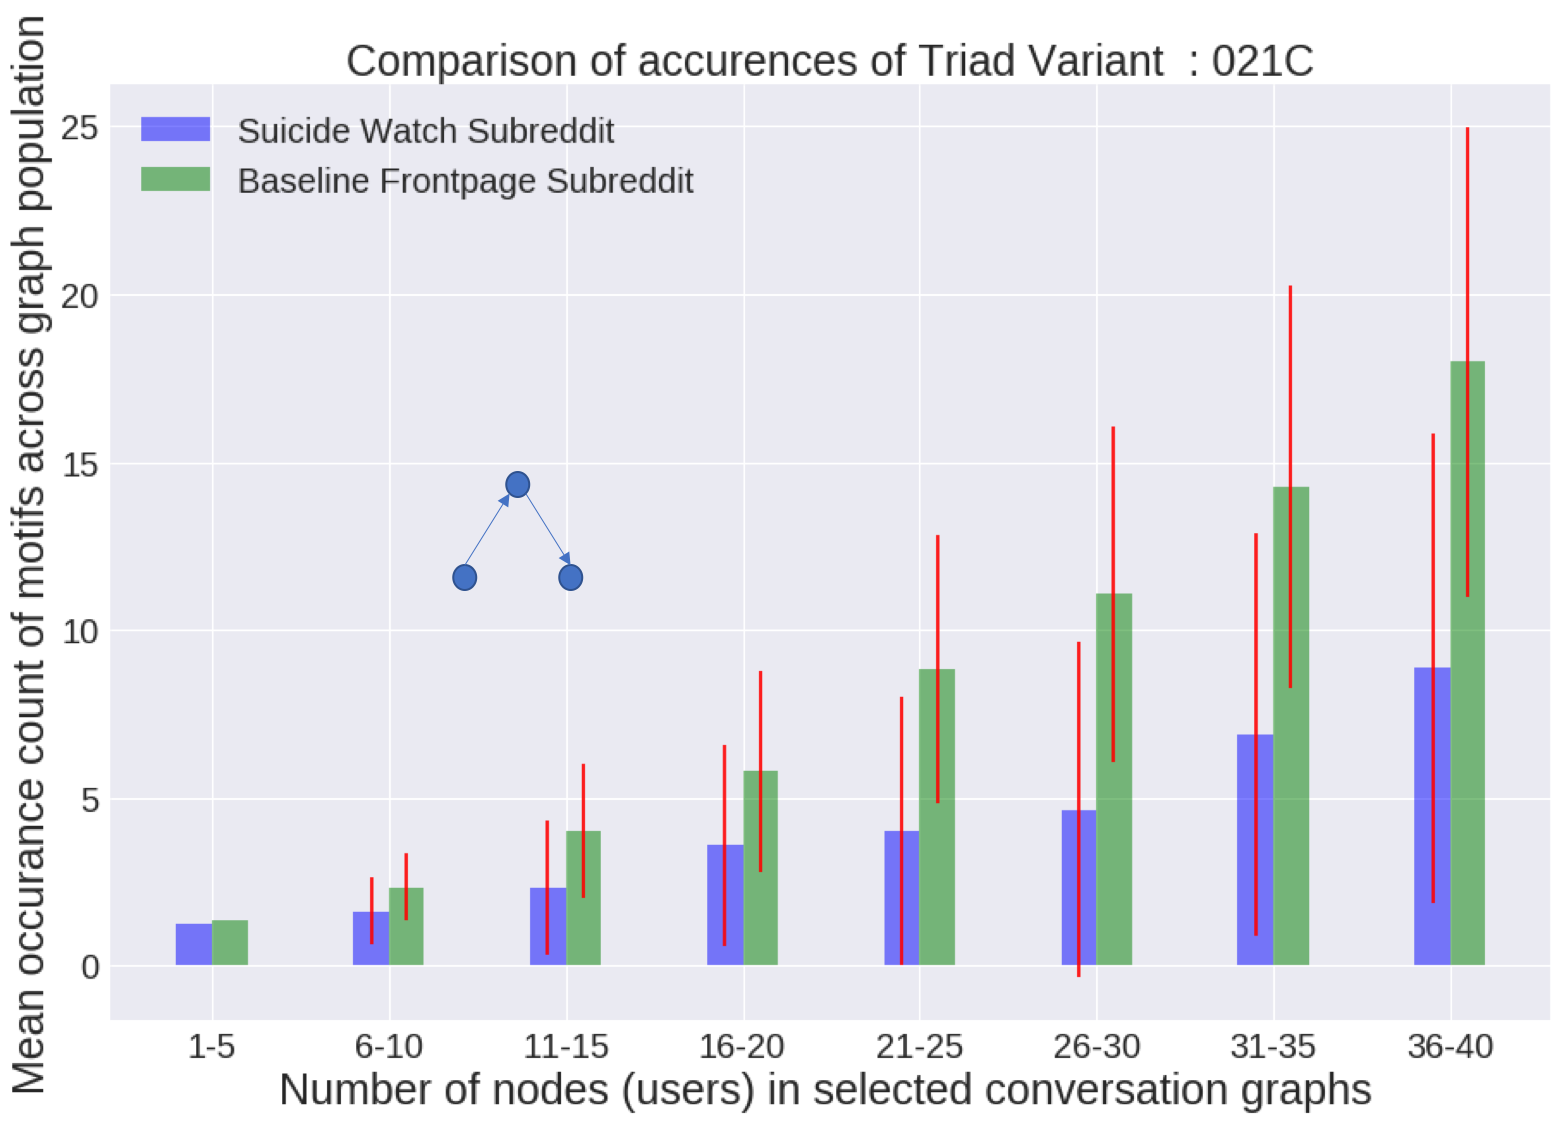
\includegraphics[width=0.33\textwidth, height = 4.5cm ]{Figures/021C}
	\label{fig:021C}
	}
	\subfloat[]{
	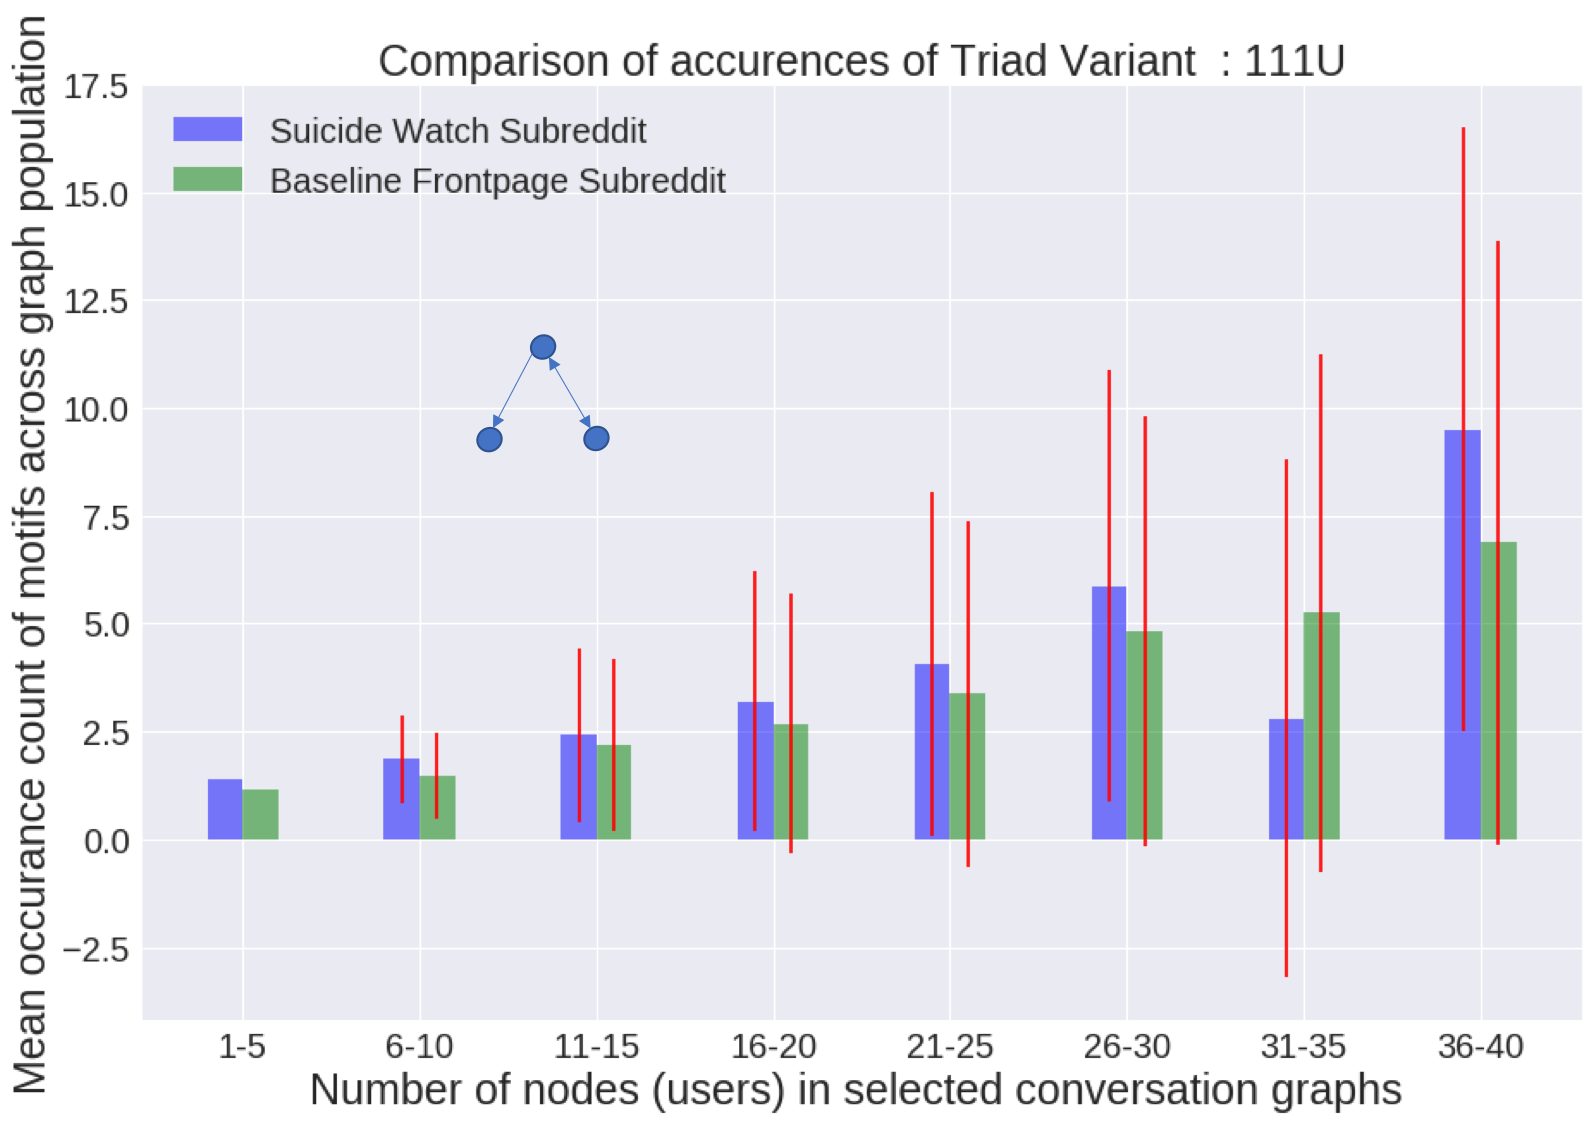
\includegraphics[width=0.33\textwidth, height = 4.5cm ]{Figures/111U}
	\label{fig:111U}
	}
    \subfloat[]{
	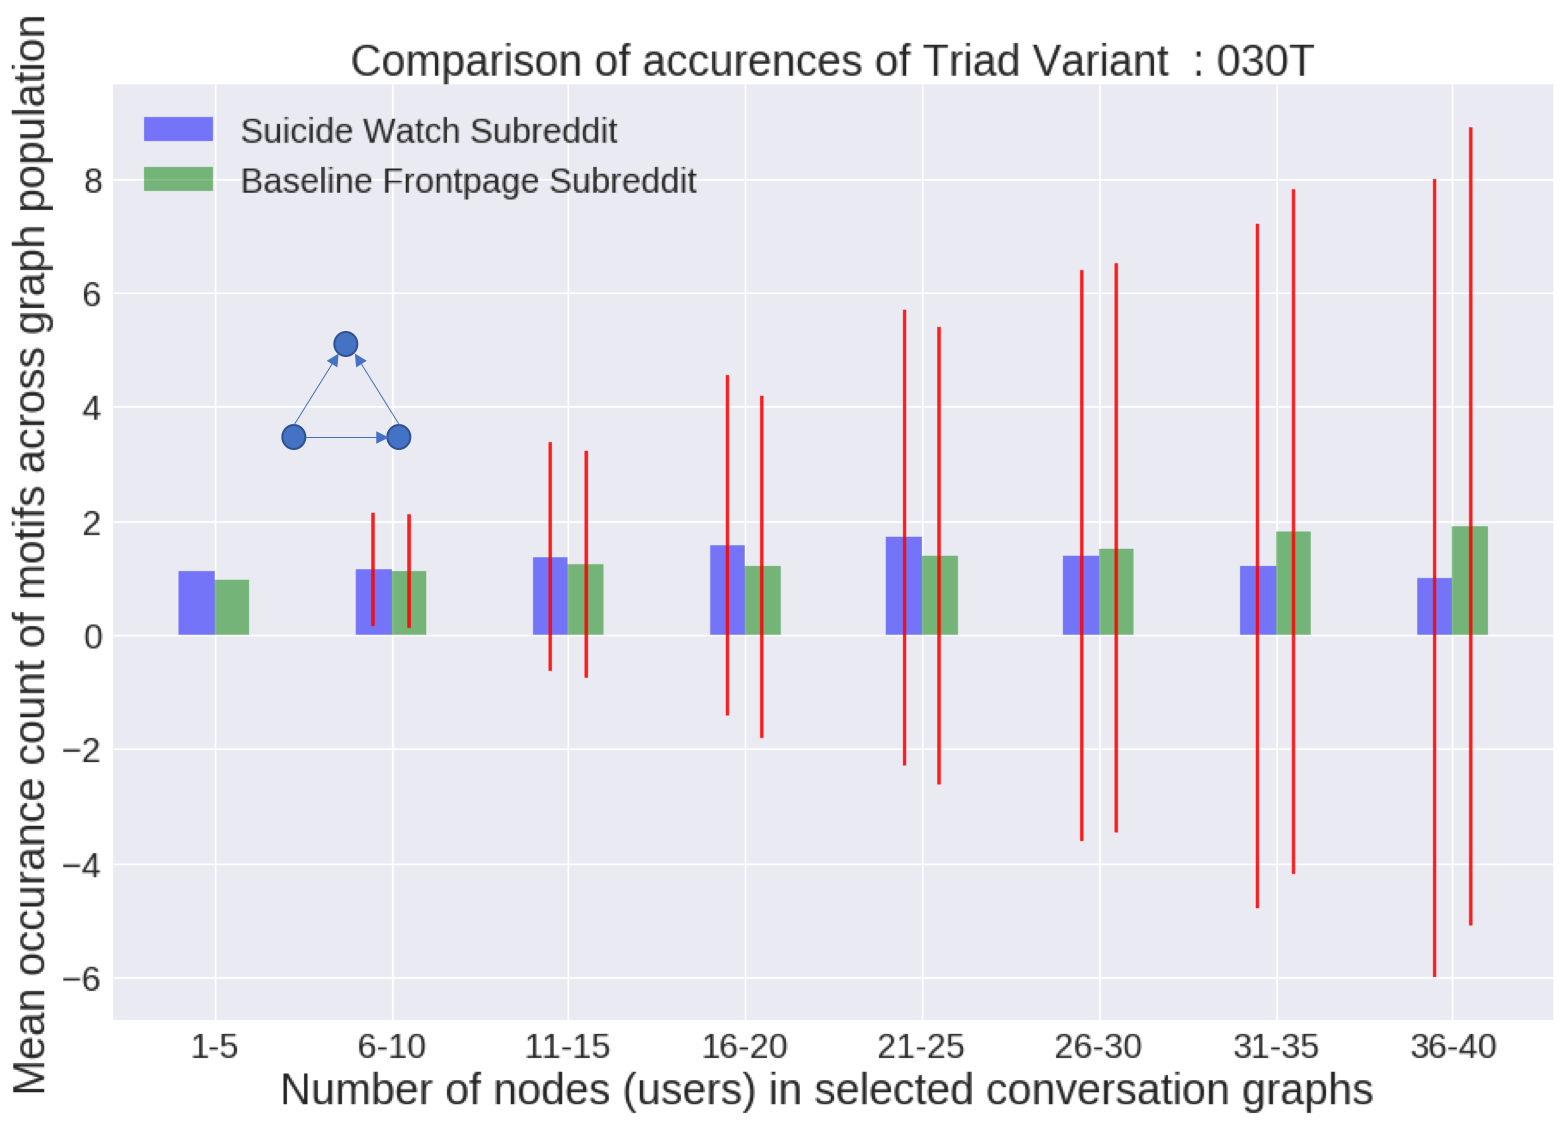
\includegraphics[width=0.33\textwidth, height = 4.5cm ]{Figures/030T}
	\label{fig:030T}
	}
	
    \subfloat[]{
	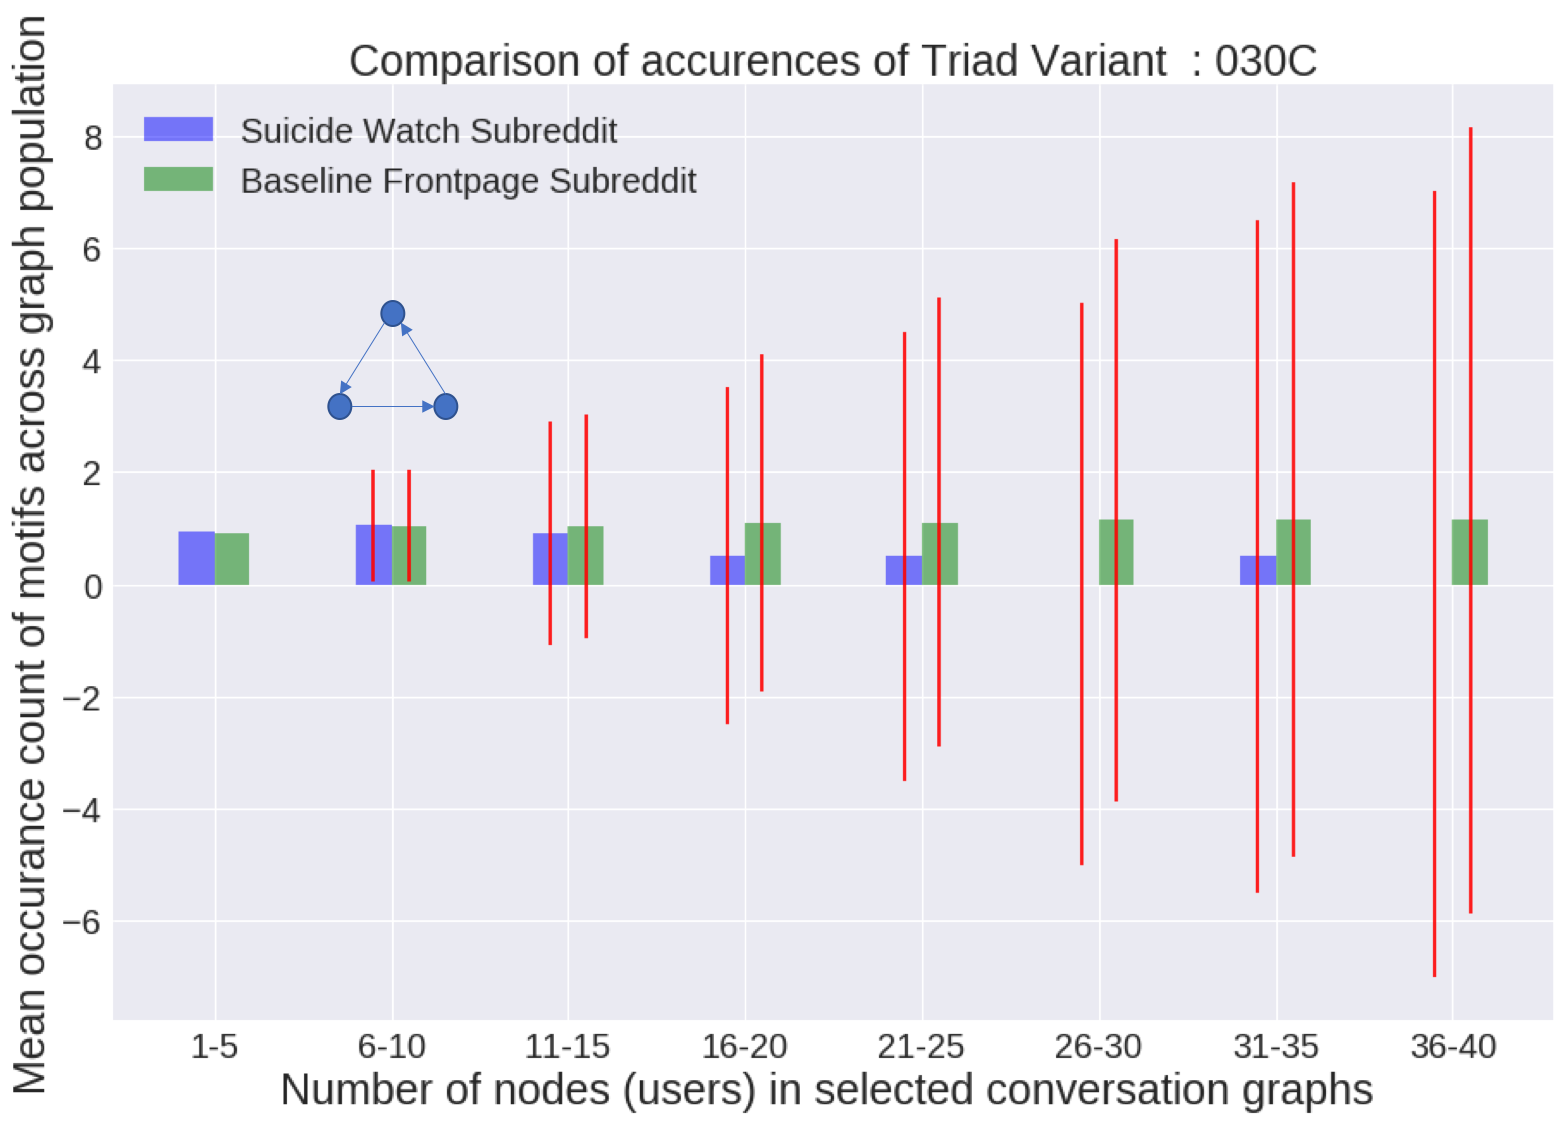
\includegraphics[width=0.33\textwidth, height = 4.5cm ]{Figures/030C}
	\label{fig:030C}
	}
	\subfloat[]{
	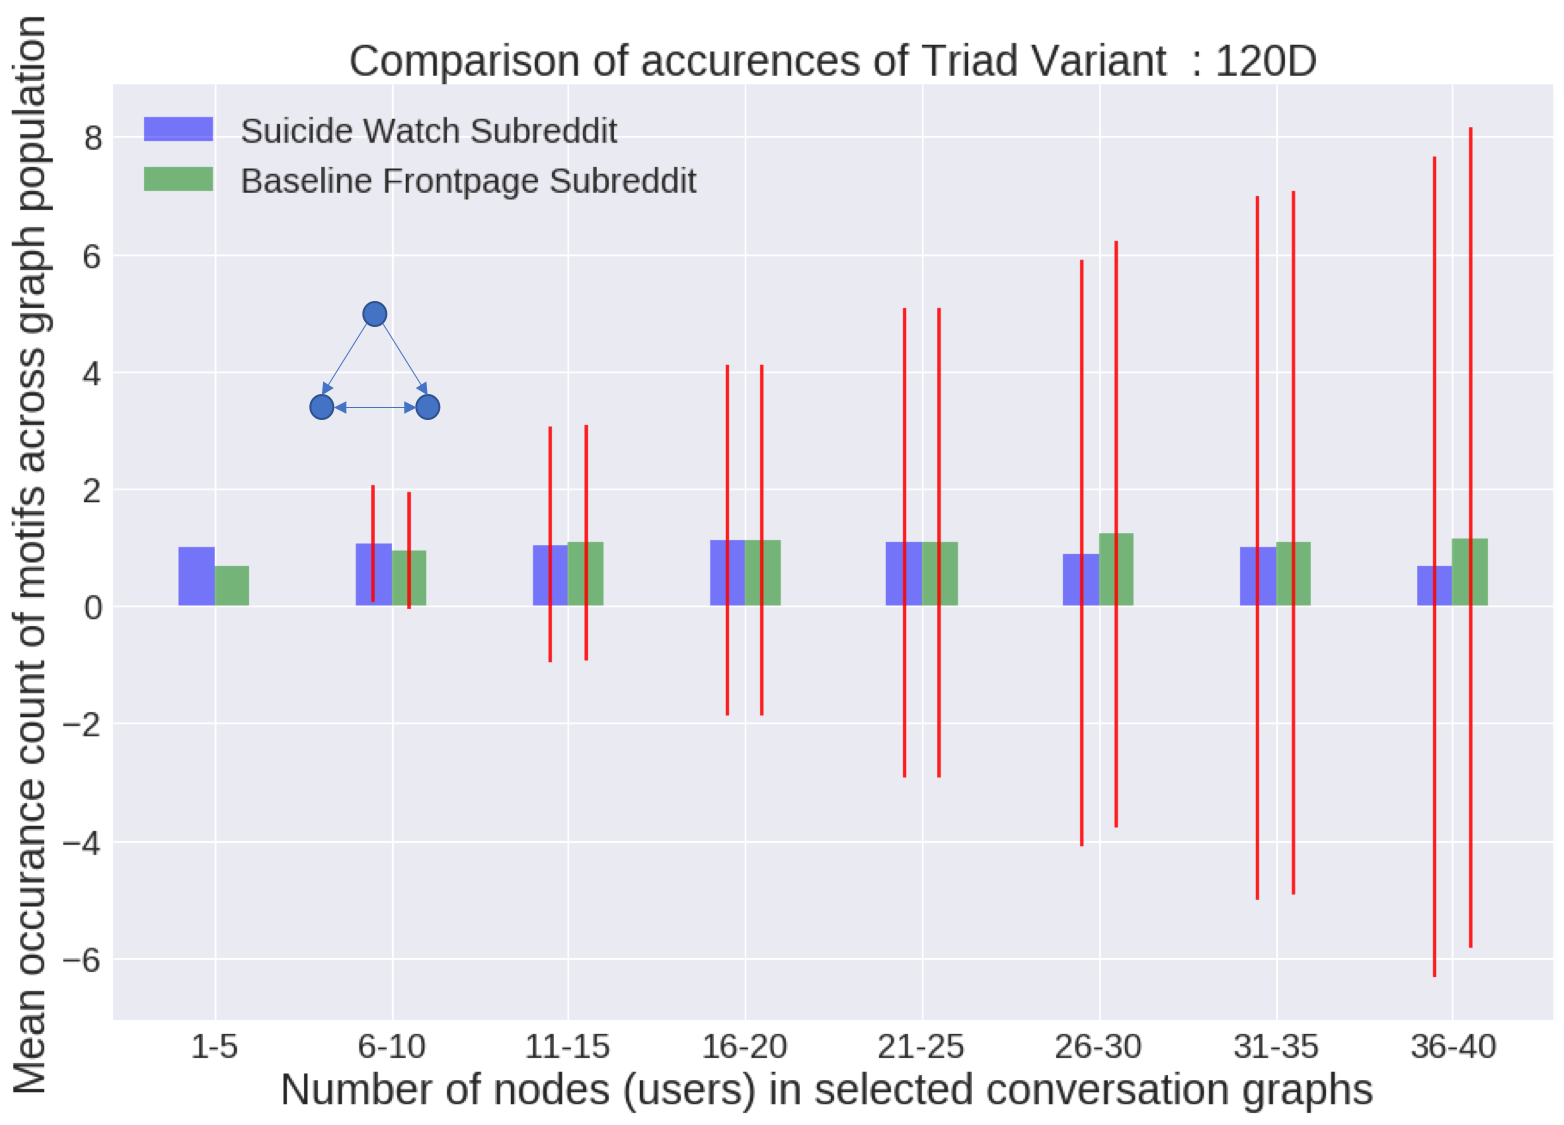
\includegraphics[width=0.33\textwidth, height = 4.5cm ]{Figures/120D}
	\label{fig:120D}
	}
    \subfloat[]{
	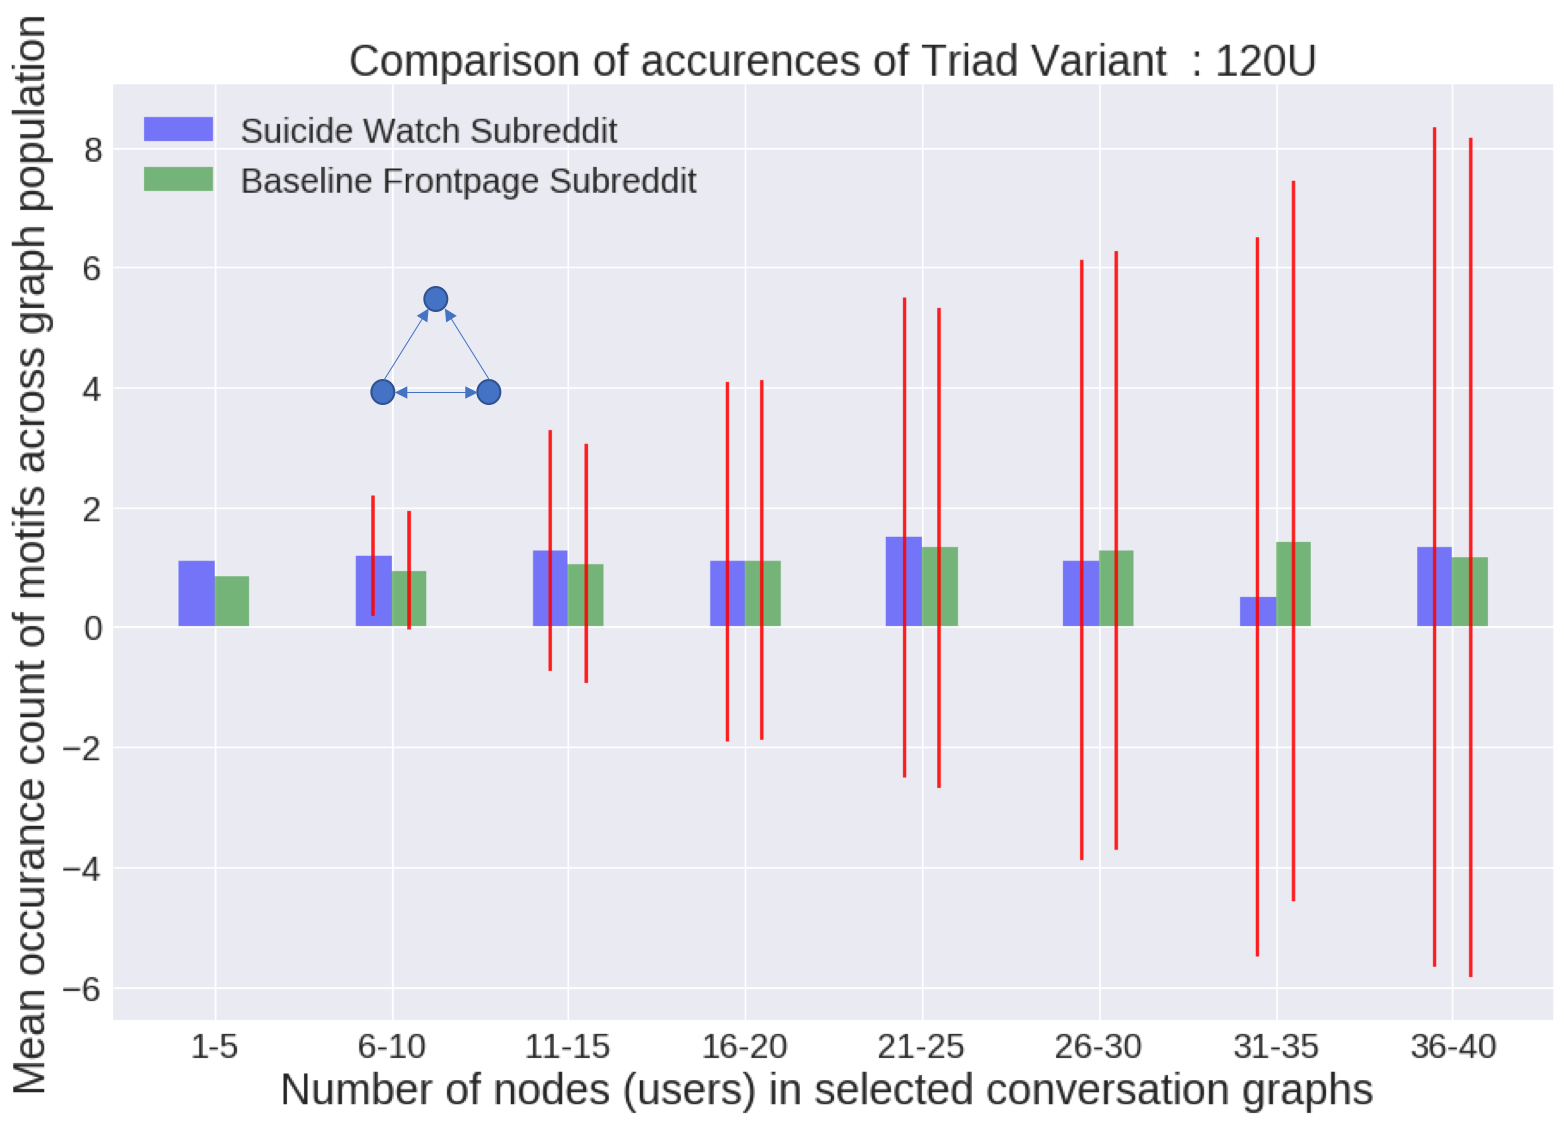
\includegraphics[width=0.3\textwidth, height = 4.5cm ]{Figures/120U}
	\label{fig:120U}
	}
    
	\subfloat[]{
	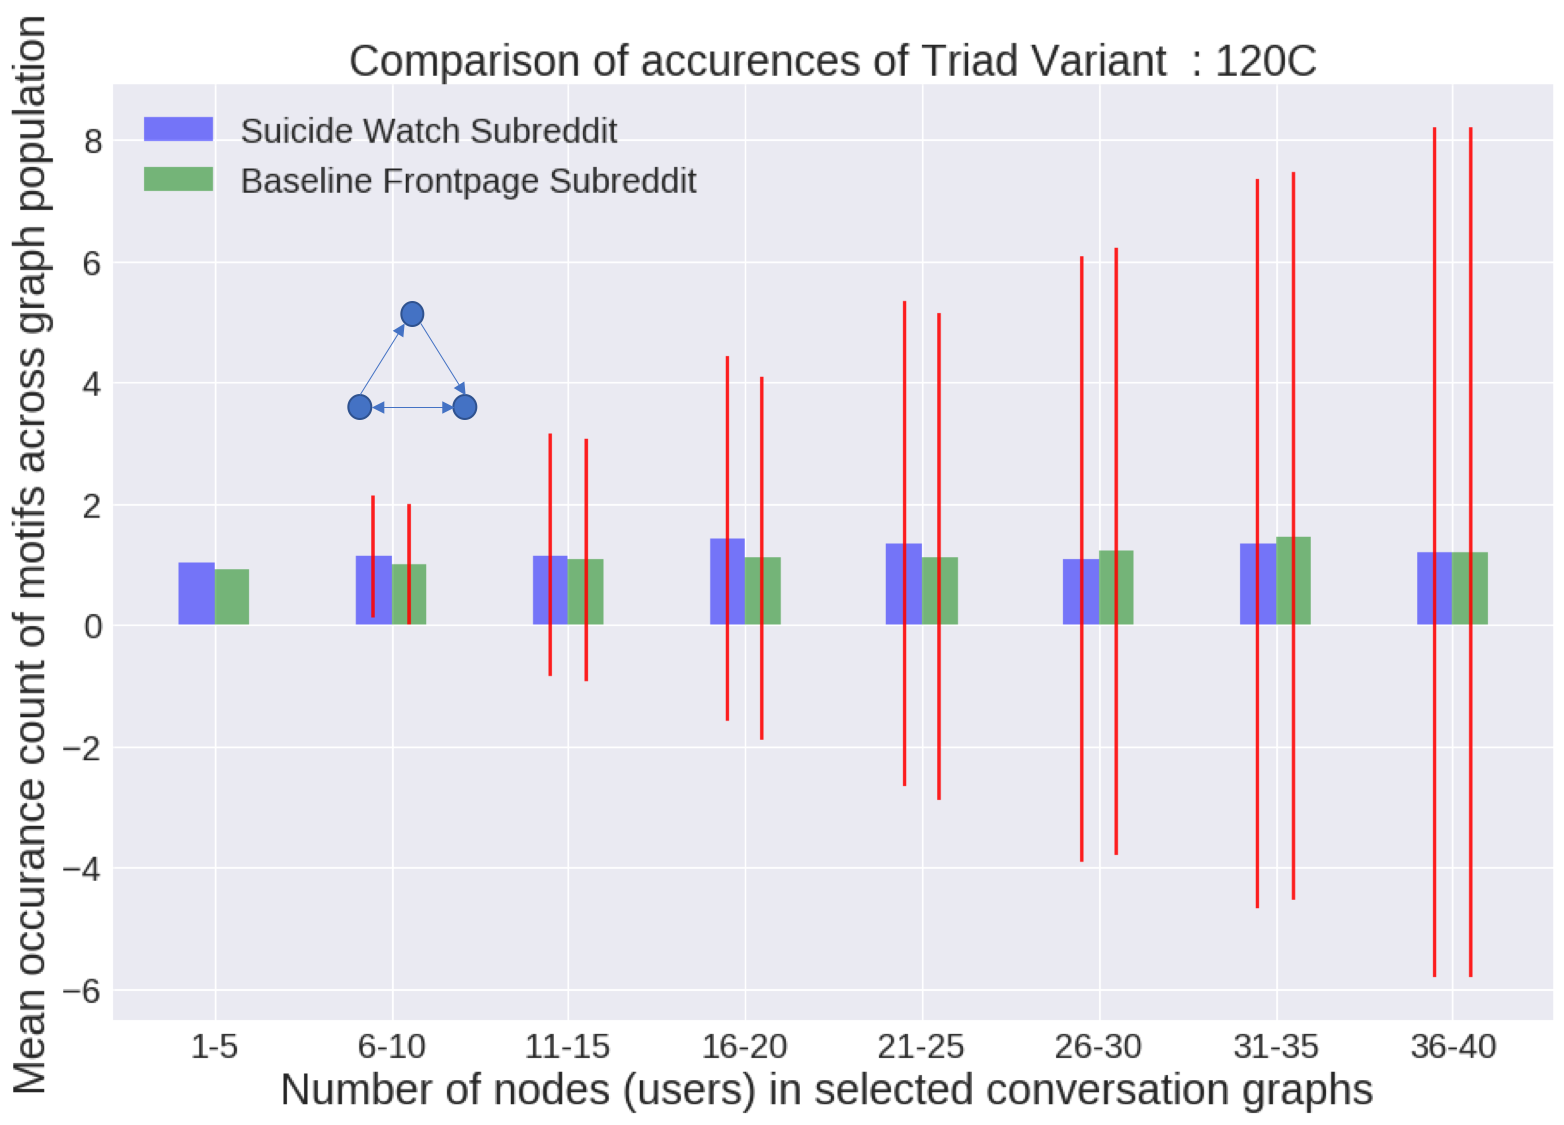
\includegraphics[width=0.33\textwidth, height = 4.5cm ]{Figures/120C}
	\label{fig:120C}
	}
	\subfloat[]{
	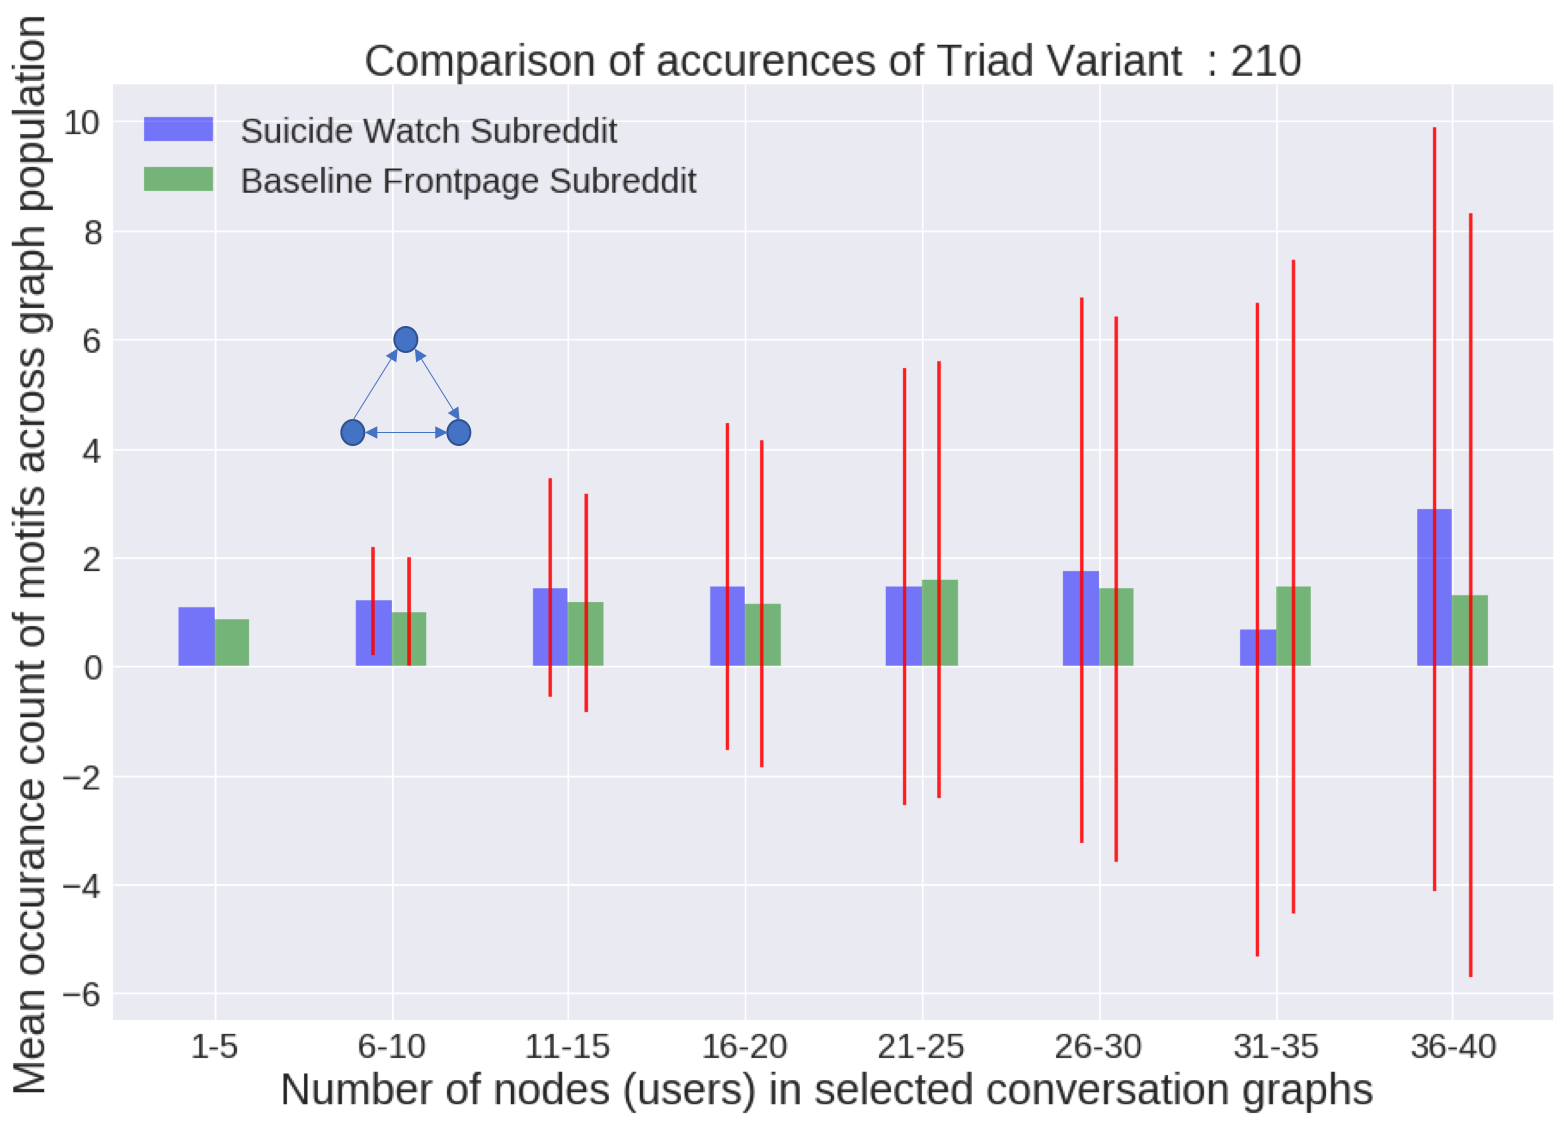
\includegraphics[width=0.33\textwidth, height = 4.5cm ]{Figures/210}
	\label{fig:210}
	}
	\subfloat[]{
	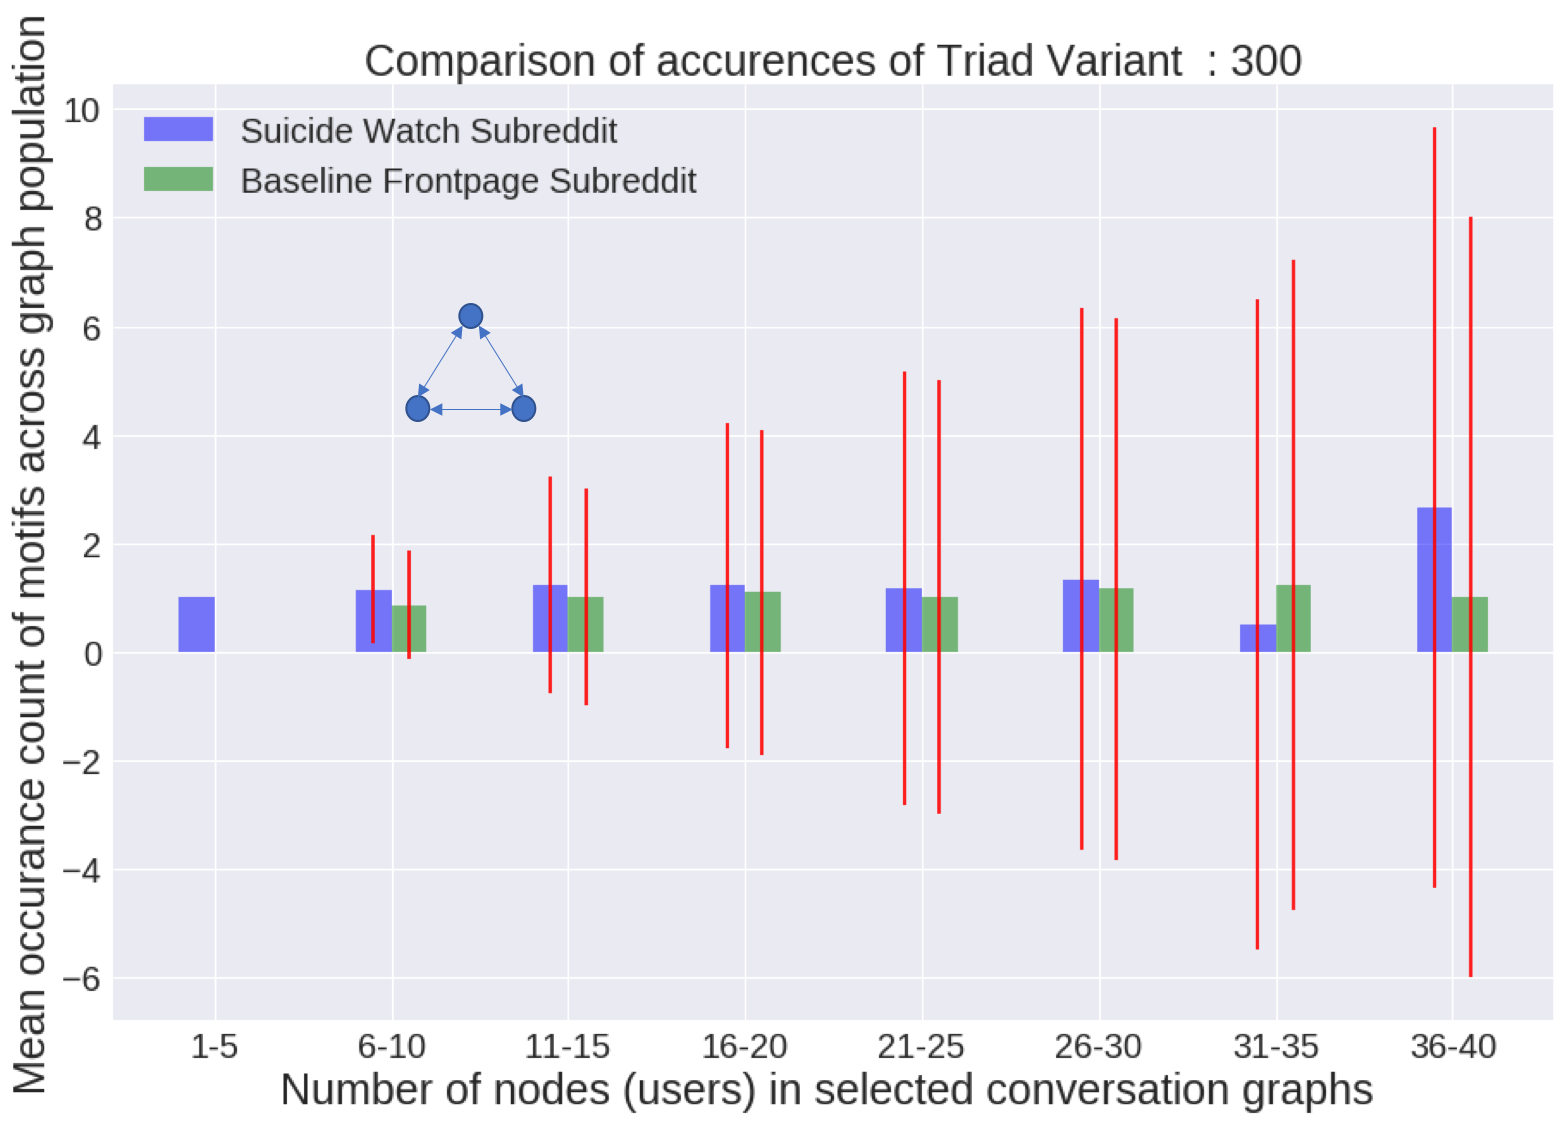
\includegraphics[width=0.33\textwidth, height = 4.5cm ]{Figures/300}
	\label{fig:300}
	}
	
	\label{fig:MotifOccurance}
	\vspace{-0.4cm}
	\caption{ The figure shows comparison of occurrence ratios of 9 insignificant motifs. Blue traces are for Suicide watch and Green traces are for Baseline Front page threads}
	\vspace{-0.4cm}
\end{figure*}


\subsection{Network characteristics}
Figure \ref{fig:depthDist} shows the distribution of maximum depths across all Reply graphs for SW and Baseline subreddits. The SW threads depths have a median depth of 2 and mean of 4 compared to median depth of 2 for BL and a mean of 2.5. This shows that statistically the depths of Suicide watch and baseline graphs are quite similar.

\begin{figure}[!ht]
    \centering
    % \hspace*{-5mm}
    \subfloat[]{
        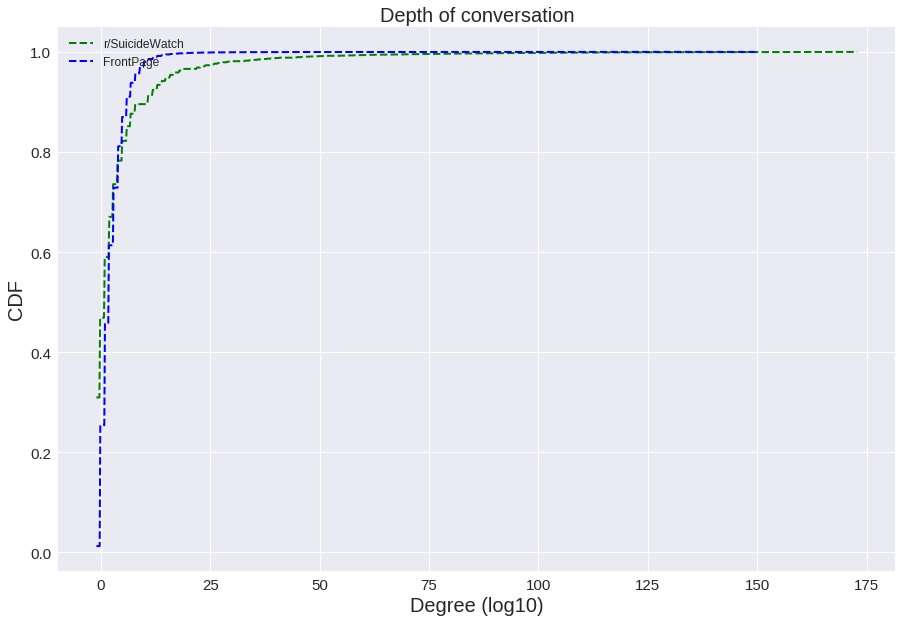
\includegraphics[width=0.4\textwidth, height = 5cm ]{Figures/DepthConversations.png}
        \label{fig:depthDist} }	
    \subfloat[]{
        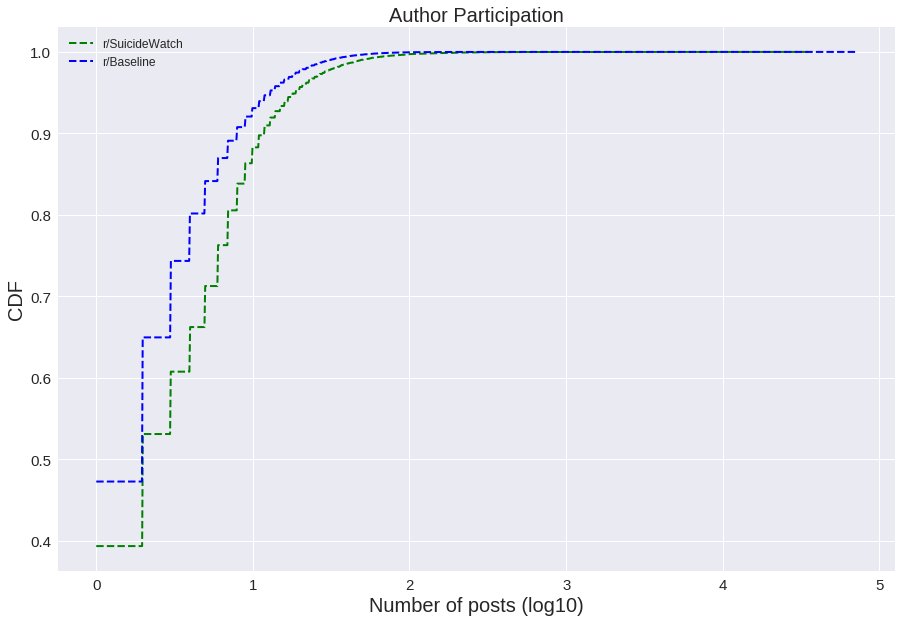
\includegraphics[width=0.4\linewidth, height = 5cm ]{Figures/AuthorParticipation.png}
        \label{fig:uniqAuthors}
    }
    
    
    \subfloat[]{
        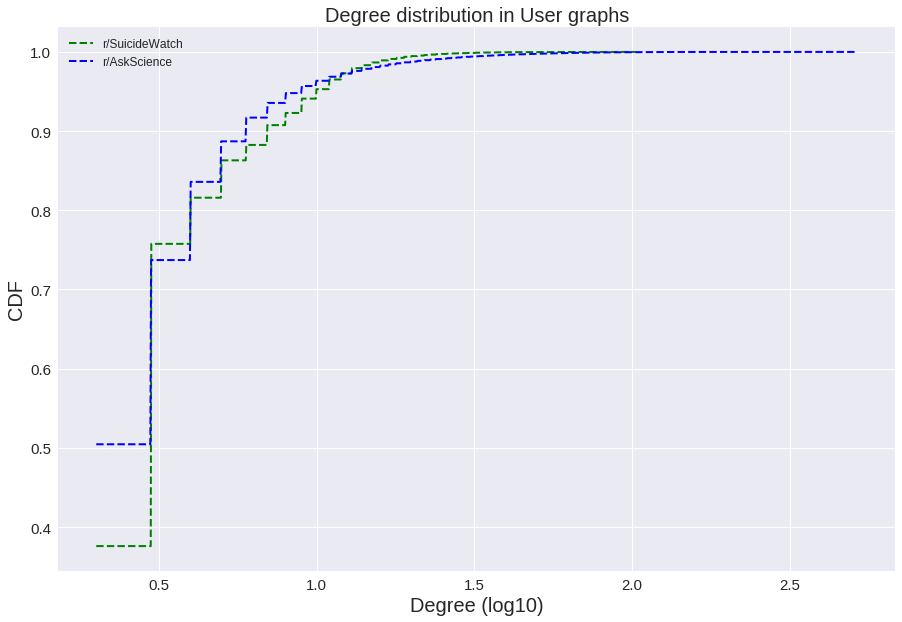
\includegraphics[width=0.4\textwidth, height = 5cm ]{Figures/degreeDistUgraph.png}
        \label{fig:degUgraph}
    }
    \subfloat[]{
        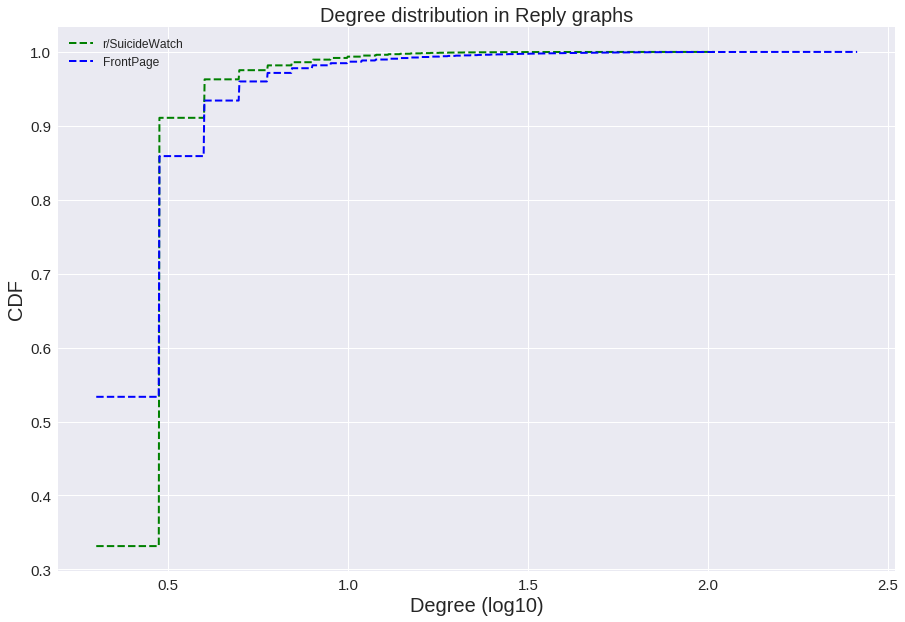
\includegraphics[width=0.4\linewidth, height = 5cm ]{Figures/degreeDistReplyGraph.png}
        \label{fig:degRgraph}
    }
    \caption{\textsl{ Fig \ref{fig:depthDist} shows the distribution of maximum depths of Reply Graphs for Subreddit r/SuicideWatch and the baseline Frontpage conversations. Fig \ref{fig:uniqAuthors} shows the distribution of unique authors per thread in the two datasets. Fig \ref{fig:degRgraph} shows Distribution of degrees for Reply Graphs,  r/SuicideWatch and FrontPage. Fig \ref{fig:degUgraph} shows the degree distributions for the reply graphs}}
\end{figure}

Figure\ref{fig:responseDist} shows the CDF for the number of responses a Root post gets on a thread across the whole dataset. 
\begin{figure}[!h]
    \centering
    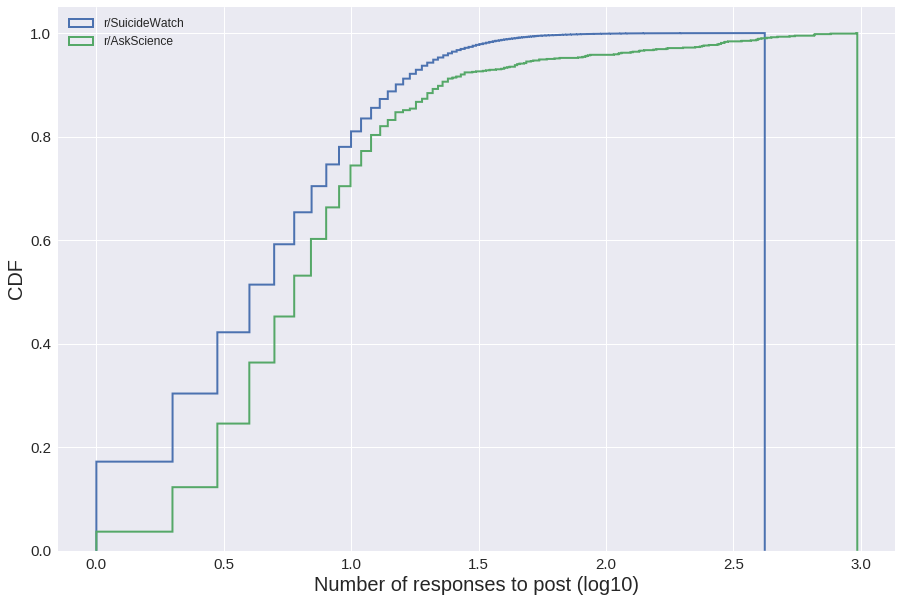
\includegraphics[width=0.4\linewidth]{Figures/responseDistSW}
    \caption{\textsl{ Distribution of responses per thread on Subreddits r/SuicideWatch and Frontpage }}
    \label{fig:responseDist}
\end{figure}
Figure \ref{fig:responseDist} shows the CDF for number of comments per thread across the r/SuicideWatch subreddit dataset and the crawled frontpage subreddit. 
